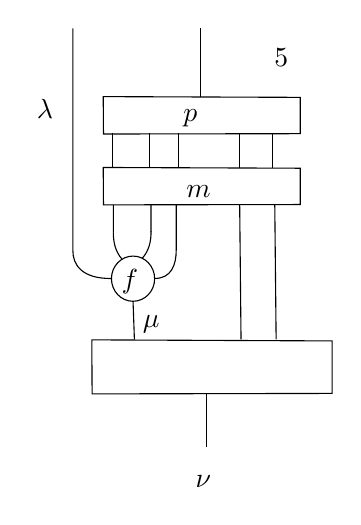
\begin{tikzpicture}[yscale=-1,scale=0.03,baseline={([yshift=-.5ex]current bounding box.center)}]
\begin{scope}[shift={(0.00mm,719.29mm)}]
% path id='path4136'
% path spec='m 348.3188,600.22405 1.19398,228.76363 1016.21342,-2.0203 0,-222.23354 z'
\draw [fill=none,draw=black] (348.32mm,600.22mm)
-- ++(1.19mm,228.76mm)
-- ++(1016.21mm,-2.02mm)
-- ++(0.00mm,-222.23mm)
-- cycle
;
% path id='path4138'
% path spec='m 974.27698,28.210035 5.71493,570.145885'
\draw [fill=none,draw=black] (974.28mm,28.21mm)
-- ++(5.71mm,570.15mm)
;
% path id='path4140'
% path spec='m 1122.8652,28.083765 5.7149,570.272155'
\draw [fill=none,draw=black] (1122.87mm,28.08mm)
-- ++(5.71mm,570.27mm)
;
% path id='path4142'
% path spec='m 522.83401,436.94502 5.76055,161.40579'
\draw [fill=none,draw=black] (522.83mm,436.95mm)
-- ++(5.76mm,161.41mm)
;
% path id='path4144'
% path spec='m 835.71429,828.07643 0,224.28587'
\draw [fill=none,draw=black] (835.71mm,828.08mm)
-- ++(0.00mm,224.29mm)
;
\node [black] at (600mm,533.02mm) { $\mu$ };
\node [black] at (820mm,1200mm) { $\nu$ };
\draw [fill=none,draw=black] (522.86mm,341.22mm) ellipse (91.43mm and 95.71mm) ;
% path id='path4227'
% path spec='M 476.35,258.6217 C 448.68273,227.90423 438.99734,187.77417 439.47944,145.48462'
\draw [fill=none,draw=black] (476.35mm,258.62mm)
%%%% Warning: check controls
.. controls (448.68mm,227.90mm) and (439.00mm,187.77mm) .. (439.48mm,145.48mm)
;
% path id='path4229'
% path spec='m 562.16133,254.45482 c 27.66727,-30.71747 37.35266,-70.84753 36.87056,-113.13708'
\draw [fill=none,draw=black] (562.16mm,254.45mm)
.. controls ++(27.67mm,-30.72mm) and ++(0.48mm,42.29mm) .. ++(36.87mm,-113.14mm)
;
% path id='path4231'
% path spec='m 614.93036,340.07385 c 69.05849,0.8629 91.19261,-57.25038 90.66119,-120.46069'
\draw [fill=none,draw=black] (614.93mm,340.07mm)
.. controls ++(69.06mm,0.86mm) and ++(0.53mm,63.21mm) .. ++(90.66mm,-120.46mm)
;
% path id='path4233'
% path spec='M 431.38448,340.52373 C 306.96687,341.38538 267.08946,283.35528 268.04688,220.23543'
\draw [fill=none,draw=black] (431.38mm,340.52mm)
%%%% Warning: check controls
.. controls (306.97mm,341.39mm) and (267.09mm,283.36mm) .. (268.05mm,220.24mm)
;
% path id='path4235'
% path spec='m 267.94657,220.77492 0.0864,-939.44957'
\draw [fill=none,draw=black] (267.95mm,220.77mm)
-- ++(0.09mm,-939.45mm)
;
% path id='path4237'
% path spec='m 705.58811,220.20895 0.0869,-191.775295'
\draw [fill=none,draw=black] (705.59mm,220.21mm)
-- ++(0.09mm,-191.78mm)
;
% path id='path4239'
% path spec='m 439.40812,146.03242 0.0868,-117.218835'
\draw [fill=none,draw=black] (439.41mm,146.03mm)
-- ++(0.09mm,-117.22mm)
;
% path id='path4241'
% path spec='m 598.97938,143.5389 0.0868,-114.877905'
\draw [fill=none,draw=black] (598.98mm,143.54mm)
-- ++(0.09mm,-114.88mm)
;
% path id='path4243'
% path spec='m 396.68171,-129.5517 0.97851,158.301765 832.82908,-1.398 0,-153.783045 z'
\draw [fill=none,draw=black] (396.68mm,-129.55mm)
-- ++(0.98mm,158.30mm)
-- ++(832.83mm,-1.40mm)
-- ++(0.00mm,-153.78mm)
-- cycle
;
\node [black] at (509.12mm,351.44mm) { $f$ };
\node [black] at (799.84mm,-29.05mm) { $m$ };
% path id='path4257'
% path spec='m 434.36559,-129.18126 0,-144.2641'
\draw [fill=none,draw=black] (434.37mm,-129.18mm)
-- ++(0.00mm,-144.26mm)
;
% path id='path4259'
% path spec='m 594.36559,-129.18126 0,-144.2641'
\draw [fill=none,draw=black] (594.37mm,-129.18mm)
-- ++(0.00mm,-144.26mm)
;
% path id='path4261'
% path spec='m 714.36559,-129.18126 0,-144.2641'
\draw [fill=none,draw=black] (714.37mm,-129.18mm)
-- ++(0.00mm,-144.26mm)
;
% path id='path4263'
% path spec='m 974.36559,-129.18126 0,-144.2641'
\draw [fill=none,draw=black] (974.37mm,-129.18mm)
-- ++(0.00mm,-144.26mm)
;
% path id='path4265'
% path spec='m 1114.3656,-129.18126 0,-144.2641'
\draw [fill=none,draw=black] (1114.37mm,-129.18mm)
-- ++(0.00mm,-144.26mm)
;
\node [black] at (150mm,-378.78mm) { $\lambda$ };
% path id='path4290'
% path spec='m 396.68171,-429.5517 0.97851,158.30178 832.82908,-1.398 0,-153.78306 z'
\draw [fill=none,draw=black] (396.68mm,-429.55mm)
-- ++(0.98mm,158.30mm)
-- ++(832.83mm,-1.40mm)
-- ++(0.00mm,-153.78mm)
-- cycle
;
\node [black] at (765.71mm,-339.07mm) { $p$ };
% path id='path4296'
% path spec='m 810,-428.35206 0,-290.71429'
\draw [fill=none,draw=black] (810.00mm,-428.35mm)
-- ++(0.00mm,-290.71mm)
;
\node [black] at (1150mm,-594.19mm) { $\ydiagram{5}$ };
\end{scope}
\end{tikzpicture}
